\documentclass[tikz,border=10pt]{standalone}
\usepackage{tikz}
\usetikzlibrary{shapes,arrows,positioning,calc,patterns,shadows,arrows.meta}

\definecolor{bertblue}{RGB}{66,133,244}
\definecolor{gptgreen}{RGB}{52,168,83}
\definecolor{unkred}{RGB}{234,67,53}
\definecolor{subwordpurple}{RGB}{142,36,245}

\begin{document}
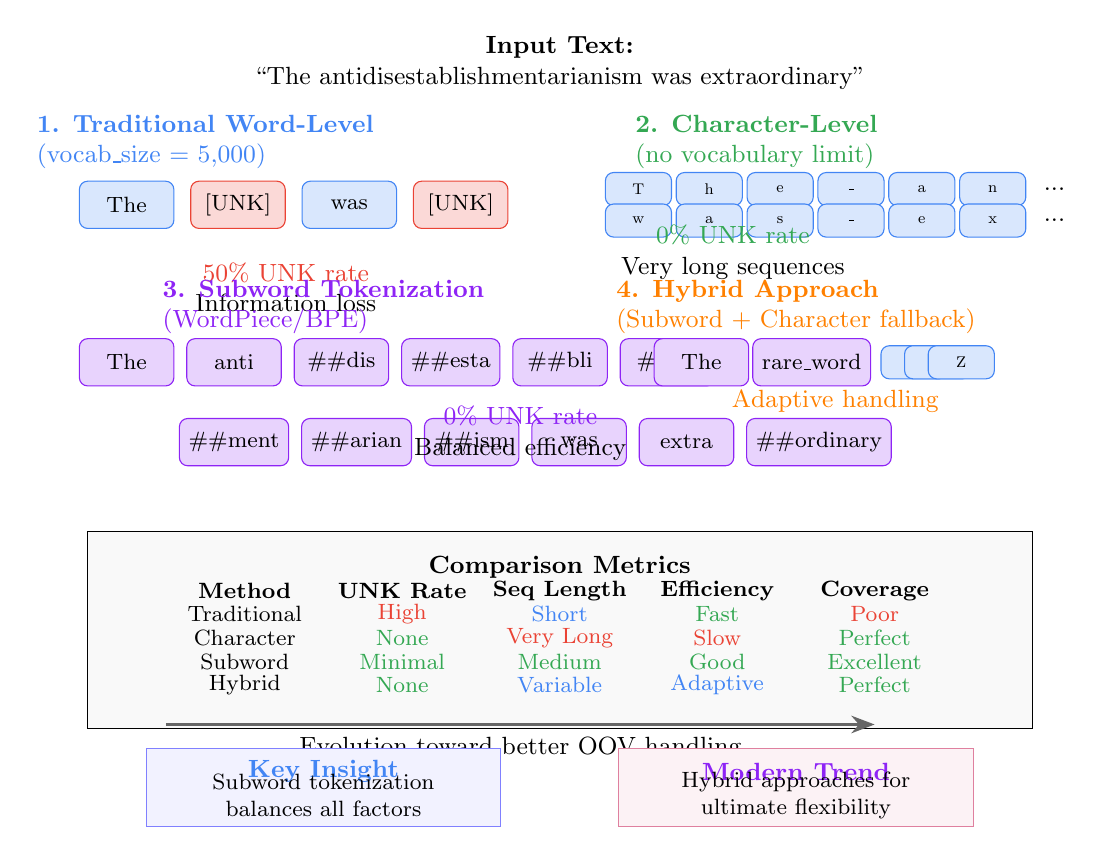
\begin{tikzpicture}[
    token/.style={rectangle, rounded corners=3pt, minimum width=1.2cm, minimum height=0.6cm, font=\footnotesize},
    unktoken/.style={token, fill=unkred!20, draw=unkred},
    goodtoken/.style={token, fill=bertblue!20, draw=bertblue},
    subword/.style={token, fill=subwordpurple!20, draw=subwordpurple},
    label/.style={font=\small},
    title/.style={font=\large\bfseries}
]

% === SPACING AND ALIGNMENT DOCUMENTATION ===
% Input text: y=8.2, centered
% Method headers: y=7.3, x positions at 1.5 and 8.5
% Token examples: y=6.5 for methods 1-2, y=4.2-3.8 for methods 3-4
% Comparison table: y=2 to 1.3
% Bottom insights: y=0

% Input text
\node[label, align=center] at (6, 9.5) {\textbf{Input Text:}\\``The antidisestablishmentarianism was extraordinary''};

% Method 1: Traditional Word-Level
\node[label, bertblue, align=left] (method1) at (1.5, 8.5) {\textbf{1. Traditional Word-Level}\\(vocab\_size = 5,000)};

\node[goodtoken] (trad1) at (0.5, 7.7) {The};
\node[unktoken, right=0.2cm of trad1] (trad2) {[UNK]};
\node[goodtoken, right=0.2cm of trad2] (trad3) {was};
\node[unktoken, right=0.2cm of trad3] (trad4) {[UNK]};

\node[label, align=center, below=0.3cm of trad2.south east] {\textcolor{unkred}{50\% UNK rate}\\Information loss};

% Method 2: Character-Level
\node[label, gptgreen, align=left] (method2) at (8.5, 8.5) {\textbf{2. Character-Level}\\(no vocabulary limit)};

% First row of characters
\node[goodtoken, scale=0.7] (char1) at (7, 7.9) {T};
\node[goodtoken, scale=0.7, right=0.05cm of char1] (char2) {h};
\node[goodtoken, scale=0.7, right=0.05cm of char2] (char3) {e};
\node[goodtoken, scale=0.7, right=0.05cm of char3] (char4) {\_};
\node[goodtoken, scale=0.7, right=0.05cm of char4] (char5) {a};
\node[goodtoken, scale=0.7, right=0.05cm of char5] (char6) {n};
\node[label, right=0.1cm of char6] {...};

% Second row of characters
\node[goodtoken, scale=0.7] (char7) at (7, 7.5) {w};
\node[goodtoken, scale=0.7, right=0.05cm of char7] (char8) {a};
\node[goodtoken, scale=0.7, right=0.05cm of char8] (char9) {s};
\node[goodtoken, scale=0.7, right=0.05cm of char9] (char10) {\_};
\node[goodtoken, scale=0.7, right=0.05cm of char10] (char11) {e};
\node[goodtoken, scale=0.7, right=0.05cm of char11] (char12) {x};
\node[label, right=0.1cm of char12] {...};

\node[label, align=center] at (8.2, 7.1) {\textcolor{gptgreen}{0\% UNK rate}\\Very long sequences};

% Method 3: Subword (BPE/WordPiece)
\node[label, subwordpurple, align=left] at (3, 6.4) {\textbf{3. Subword Tokenization}\\(WordPiece/BPE)};

% First word breakdown - properly spaced with more room
\node[subword] (sub1) at (0.5, 5.7) {The};
\node[subword, right=0.15cm of sub1] (sub2) {anti};
\node[subword, right=0.15cm of sub2] (sub3) {\#\#dis};
\node[subword, right=0.15cm of sub3] (sub4) {\#\#esta};
\node[subword, right=0.15cm of sub4] (sub5) {\#\#bli};
\node[subword, right=0.15cm of sub5] (sub6) {\#\#sh};

% Second row of subwords with better spacing
\node[subword, below=0.4cm of sub2] (sub7) {\#\#ment};
\node[subword, right=0.15cm of sub7] (sub8) {\#\#arian};
\node[subword, right=0.15cm of sub8] (sub9) {\#\#ism};
\node[subword, right=0.15cm of sub9] (sub10) {was};
\node[subword, right=0.15cm of sub10] (sub11) {extra};
\node[subword, right=0.15cm of sub11] (sub12) {\#\#ordinary};

\node[label, align=center] at (5.5, 4.8) {\textcolor{subwordpurple}{0\% UNK rate}\\Balanced efficiency};

% Method 4: Hybrid Approach
\node[label, color=orange, align=left] at (9, 6.4) {\textbf{4. Hybrid Approach}\\(Subword + Character fallback)};

\node[subword] at (7.8, 5.7) {The};
\node[subword] at (9.2, 5.7) {rare\_word};
\node[goodtoken, scale=0.7] at (10.5, 5.7) {X};
\node[goodtoken, scale=0.7] at (10.8, 5.7) {Y};
\node[goodtoken, scale=0.7] at (11.1, 5.7) {Z};

\node[label, align=center] at (9.5, 5.2) {\textcolor{orange}{Adaptive handling}};

% Comparison metrics - moved down to avoid overlap
\node[rectangle, draw=black, fill=gray!5, minimum width=12cm, minimum height=2.5cm] at (6, 2.3) {};
\node[label, font=\small\bfseries] at (6, 3.1) {Comparison Metrics};

% Table headers
\node[label, font=\footnotesize\bfseries] at (2, 2.8) {Method};
\node[label, font=\footnotesize\bfseries] at (4, 2.8) {UNK Rate};
\node[label, font=\footnotesize\bfseries] at (6, 2.8) {Seq Length};
\node[label, font=\footnotesize\bfseries] at (8, 2.8) {Efficiency};
\node[label, font=\footnotesize\bfseries] at (10, 2.8) {Coverage};

% Row 1: Traditional
\node[label, font=\footnotesize] at (2, 2.5) {Traditional};
\node[label, font=\footnotesize, unkred] at (4, 2.5) {High};
\node[label, font=\footnotesize, bertblue] at (6, 2.5) {Short};
\node[label, font=\footnotesize, gptgreen] at (8, 2.5) {Fast};
\node[label, font=\footnotesize, unkred] at (10, 2.5) {Poor};

% Row 2: Character
\node[label, font=\footnotesize] at (2, 2.2) {Character};
\node[label, font=\footnotesize, gptgreen] at (4, 2.2) {None};
\node[label, font=\footnotesize, unkred] at (6, 2.2) {Very Long};
\node[label, font=\footnotesize, unkred] at (8, 2.2) {Slow};
\node[label, font=\footnotesize, gptgreen] at (10, 2.2) {Perfect};

% Row 3: Subword
\node[label, font=\footnotesize] at (2, 1.9) {Subword};
\node[label, font=\footnotesize, gptgreen] at (4, 1.9) {Minimal};
\node[label, font=\footnotesize, gptgreen] at (6, 1.9) {Medium};
\node[label, font=\footnotesize, gptgreen] at (8, 1.9) {Good};
\node[label, font=\footnotesize, gptgreen] at (10, 1.9) {Excellent};

% Row 4: Hybrid
\node[label, font=\footnotesize] at (2, 1.6) {Hybrid};
\node[label, font=\footnotesize, gptgreen] at (4, 1.6) {None};
\node[label, font=\footnotesize, bertblue] at (6, 1.6) {Variable};
\node[label, font=\footnotesize, bertblue] at (8, 1.6) {Adaptive};
\node[label, font=\footnotesize, gptgreen] at (10, 1.6) {Perfect};

% Evolution arrow
\draw[-{Stealth}, very thick, black!60] (1, 1.1) -- (10, 1.1);
\node[label] at (5.5, 0.8) {Evolution toward better OOV handling};

% Key insights - better spaced
\node[rectangle, draw=blue!50, fill=blue!5, minimum width=4.5cm, minimum height=1cm] at (3, 0.3) {};
\node[label, font=\small\bfseries, bertblue] at (3, 0.5) {Key Insight};
\node[label, font=\footnotesize, align=center] at (3, 0.2) {Subword tokenization\\balances all factors};

\node[rectangle, draw=purple!50, fill=purple!5, minimum width=4.5cm, minimum height=1cm] at (9, 0.3) {};
\node[label, font=\small\bfseries, subwordpurple] at (9, 0.5) {Modern Trend};
\node[label, font=\footnotesize, align=center] at (9, 0.2) {Hybrid approaches for\\ultimate flexibility};

\end{tikzpicture}
\end{document}